\documentclass[a4paper, 10pt]{article}

\usepackage[english]{babel}
\usepackage[utf8]{inputenc}
\usepackage{amsmath}
\usepackage{graphicx}
\usepackage[colorinlistoftodos]{todonotes}
\usepackage{amsmath}
\usepackage{array}
\usepackage{multirow}
\usepackage{graphicx}
\usepackage{epstopdf}
%\usepackage{subfigure}
\usepackage{subcaption}
\usepackage{tikz}
\usepackage{pgfplots}
\usepackage[colorinlistoftodos]{todonotes}
\usepackage[colorlinks=true, allcolors=blue]{hyperref}
\usepackage{placeins}
\usetikzlibrary{arrows}
\usetikzlibrary{intersections}
\usepgfplotslibrary{fillbetween}
\usepackage{setspace}

\DeclareGraphicsExtensions{.eps,.pdf,.png,.tikz}
\graphicspath{{figs/}}

\newcolumntype{M}[1]{>{\centering\arraybackslash}m{#1}}
\renewcommand\thefootnote{\textcolor{red}{\arabic{footnote}}}

\DeclareRobustCommand\sampleline[1]{%
	\tikz\draw[#1] (0,0) (0,\the\dimexpr\fontdimen22\textfont2\relax)
	-- (2em,\the\dimexpr\fontdimen22\textfont2\relax);%
}

\title{Hebbian-LMS vs Backpropagation}

%\author{JKP}

\date{\today}

\begin{document}
\maketitle

\section*{Definitions}

\begin{itemize}
	\item Centroids are distributed according to a Gaussian distribution with zero mean and unit variance ($\mathcal{N}(0, 1)$)
	\item The patterns are distributed about the centroid according to a Gaussian distribution with variance $\sigma^2$ ($\mathcal{N}(0, \sigma^2)$)
	\item The difficulty of the classification problem is characterized by the parameter $\rho$:
	\begin{equation}
	\rho = \frac{\text{standard deviation of patterns in a cluster } (\sigma)}{\text{average distance between centroids}} 
	\end{equation}
	From properties of $\chi$-square distribution, it can be shown that 
	\begin{equation}
	\rho = \frac{\sigma}{\sqrt{2N}},
	\end{equation} 
	where $N$ is the number of dimensions of the input space.
\end{itemize}

Unless otherwise specified, the results presented in the following sections assume the parameters listed in Table~\ref{tab:param}.

\begin{table}[!h]
	\centering
	\caption{Simulation parameters.} \label{tab:param}.
	\begin{tabular}{c|c}
		\hline
		Parameter & Value \\
		\hline
		Number of inputs ($N$) & 50 \\
		Number of hidden layers & 3 \\
		% Number of neurons per hidden layer & 150 \\
		Number of clusters & 100 \\
		Number of input patterns per cluster & 50 \\
		Training set & 150 patterns/cluster \\
		Test set & 50 patterns/cluster \\		 
		Output layer function & softmax / one-out-of-many \\
		Adaptation constant & $\mu = 0.1/N = 10^{-3}$ \\
		Standard deviation of initial weights ($\sigma_W)$ & $\sigma_W \approx (2\gamma\sqrt{N})^{-1} = 0.1667$ \\
		Slope in HLMS neuron ($\gamma$) & $\gamma = 0.3$ \\
		\hline
	\end{tabular}
\end{table}

\newpage
\section*{Regular network: 150 neurons per hidden layer}

\FloatBarrier
\begin{figure}[h!]
	\centering
	\begin{subfigure}[h!]{0.75\textwidth}
		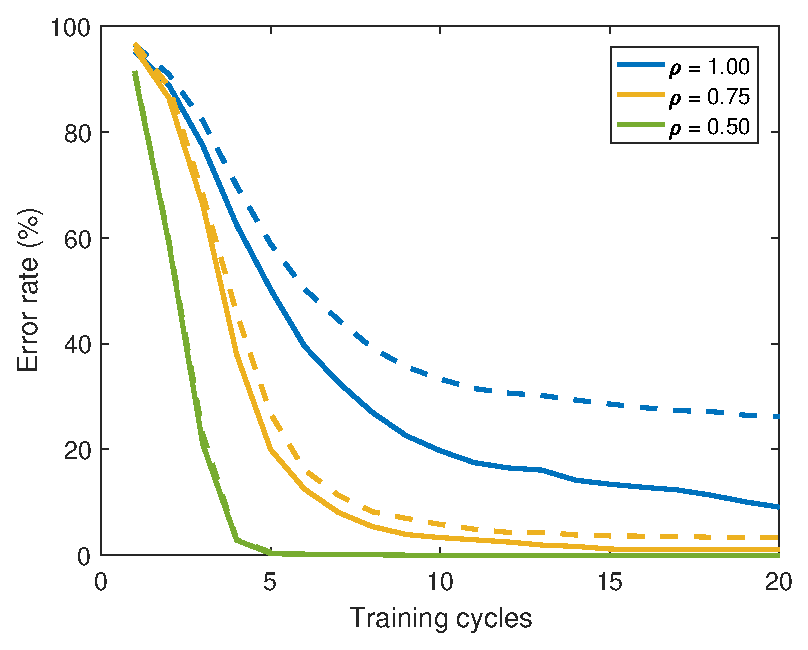
\includegraphics[width=\textwidth]{figs/rho_hlms.eps}
		\caption{HLMS}
	\end{subfigure}%
	
	\begin{subfigure}[h!]{0.75\textwidth}
		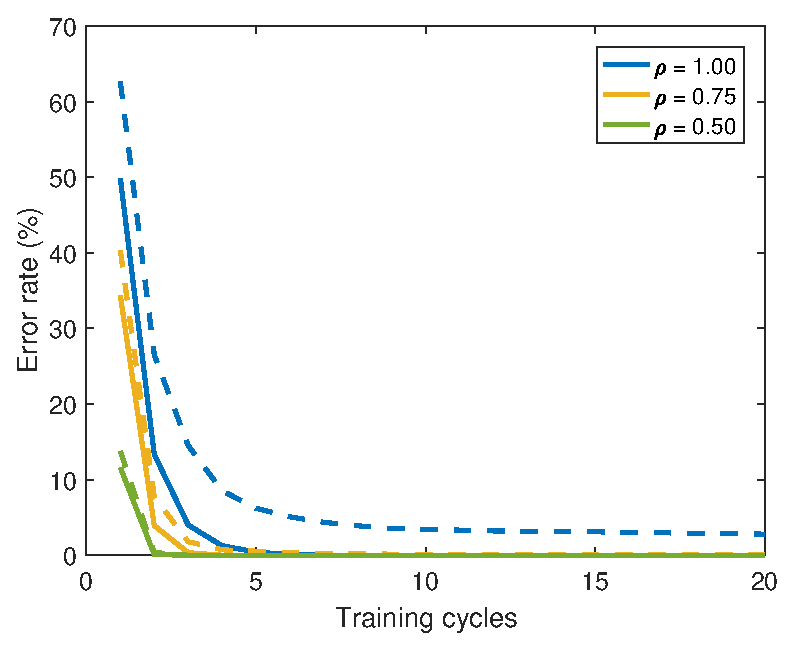
\includegraphics[width=\textwidth]{rho_bp.eps}
		\caption{Backpropagation}
	\end{subfigure}
	\caption{Learning curves for several values of $\rho$ for (a) HLMS and (b) backpropagation. All parameters are as listed in Table~\ref{tab:param}. Solid lines (\sampleline{}) correspond to training error, while dashed lines (\sampleline{dashed}) correspond to test error.} \label{fig:rho}
\end{figure}
\FloatBarrier
\newpage

\section*{Wide network: 1000 neuron per hidden layer}

\FloatBarrier
\begin{figure}[h!]
	\centering
	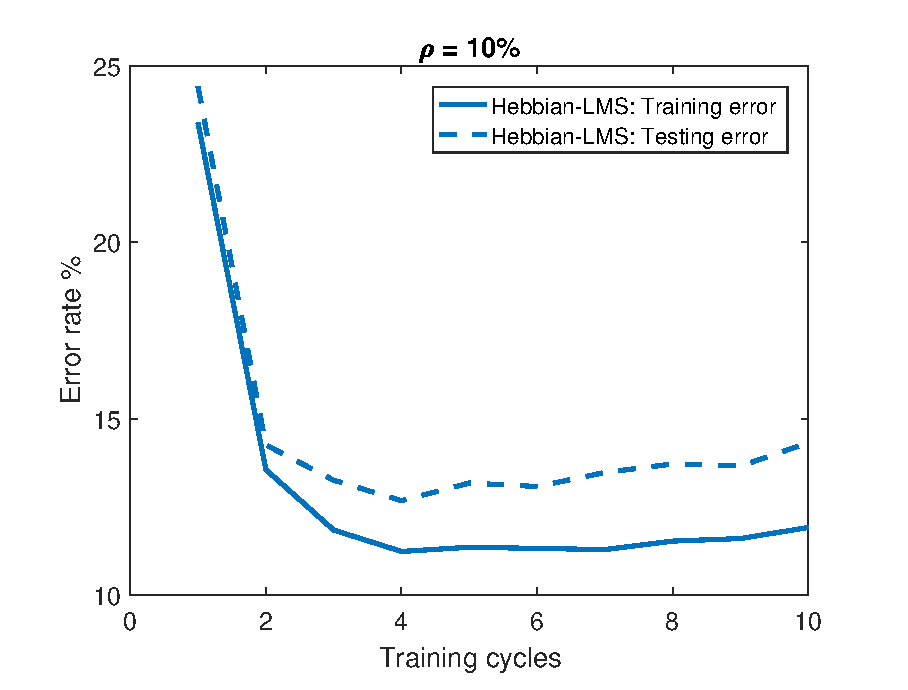
\includegraphics[width=\textwidth]{figs/wide_net.eps}
	\caption{Learning curve of HLMS for $\rho = 10\%$. A wide network of 1000 neurons/hidden layer exhibit slightly better performance than a network with only 150 neurons/hidden layer shown in Fig.~\ref{fig:rho}.} \label{fig:wide}
\end{figure}
\FloatBarrier

\newpage
\section*{Tests with MNIST data set}

\begin{itemize}
 	\item Training set is comprised of 60000 images of $28 \times 28$ hand-written digits.
 	\item Testing set is comprised of 10000 images of $28 \times 28$ hand-written digits. Fig.~\ref{fig:mnist} shows 9 random samples from the test set.
\end{itemize}

\begin{figure}[h!]
	\centering
	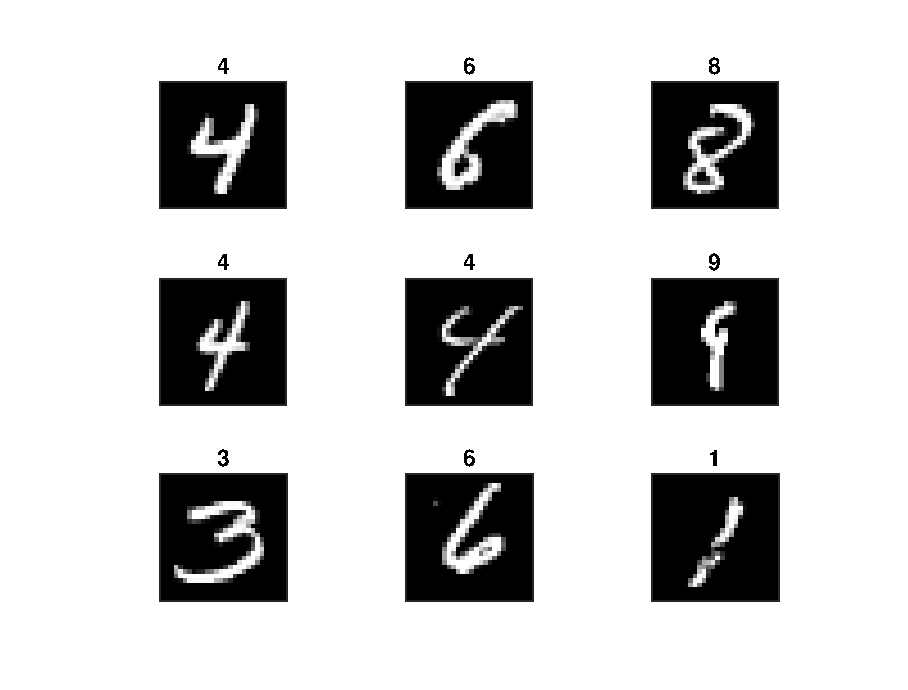
\includegraphics[width=\textwidth]{figs/mnist-samples.eps}
	\caption{Sample of 9 digits from the test set.} \label{fig:mnist}
\end{figure}

I tested different network architectures trained with HLMS and backprop on the MNIST data set. The results are summarized in Table~\ref{tab:mnist}. Backprop exhibits much better performance. Making the network wider helps HLMS only slightly. Table~\ref{tab:mnist} also shows some of the best published results obtained in the MNIST data set using deep dense and convolutional neural nets. 

\begin{table}[h!]
	\centering
	\caption{Performance comparison. For all cases the networks had $28 \times 28 = 784$ inputs and 10 outputs.} \label{tab:mnist}
	\begin{tabular}{c|p{7cm}|c}
		\hline
		Algorithm & Network & Test error rate ($\%$) \\
		\hline
		\multirow{3}{*}{HLMS} & 3 hidden layers of 300 neurons & 50 \\
		& 3 hidden layers of 1500 neurons & 43 \\
		& 5 hidden layers of 1500 neurons & 66 \\
		\hline
		Backprop & 2 hidden layers of 300 neurons & 2.5 \\
		\hline
		\multicolumn{3}{c}{Best published results on this data set} \\
		\hline
		\multirow{2}{*}{Backprop} & 6-layer fully connected network (neurons/layer: 784-2500-2000-1500-1000-500-10) & 0.35 \\
		 & 8-layer convolutional network & 0.35 \\
		\hline
	\end{tabular}
\end{table}

\end{document}